%this file is the second report
%a % comment anything after % until the end of the line

%minimum references to begin our article
\documentclass[12pt]{article}
\usepackage[english]{babel}
\usepackage[utf8]{inputenc}
\usepackage[T1]{fontenc}
\usepackage{graphicx}
\usepackage{fancyhdr}
\usepackage{hyperref}
\usepackage{float}
\usepackage{enumitem}
\usepackage{amsmath}
\usepackage[margin=1in]{geometry}
\usepackage{indentfirst}
\usepackage{titlesec}
\usepackage{verbatim}
\usepackage{url}
\usepackage{subfig}
\usepackage{float}
\usepackage{pdfpages}
\newcommand{\sectionbreak}{\clearpage}
\begin{document}
\section{Introduction}	


\subsubsection{Gantt diagram}
\clearpage
\begin{figure}[htb]
\begin{center} %angle = 90 pour pivoter
\makebox[\textwidth]{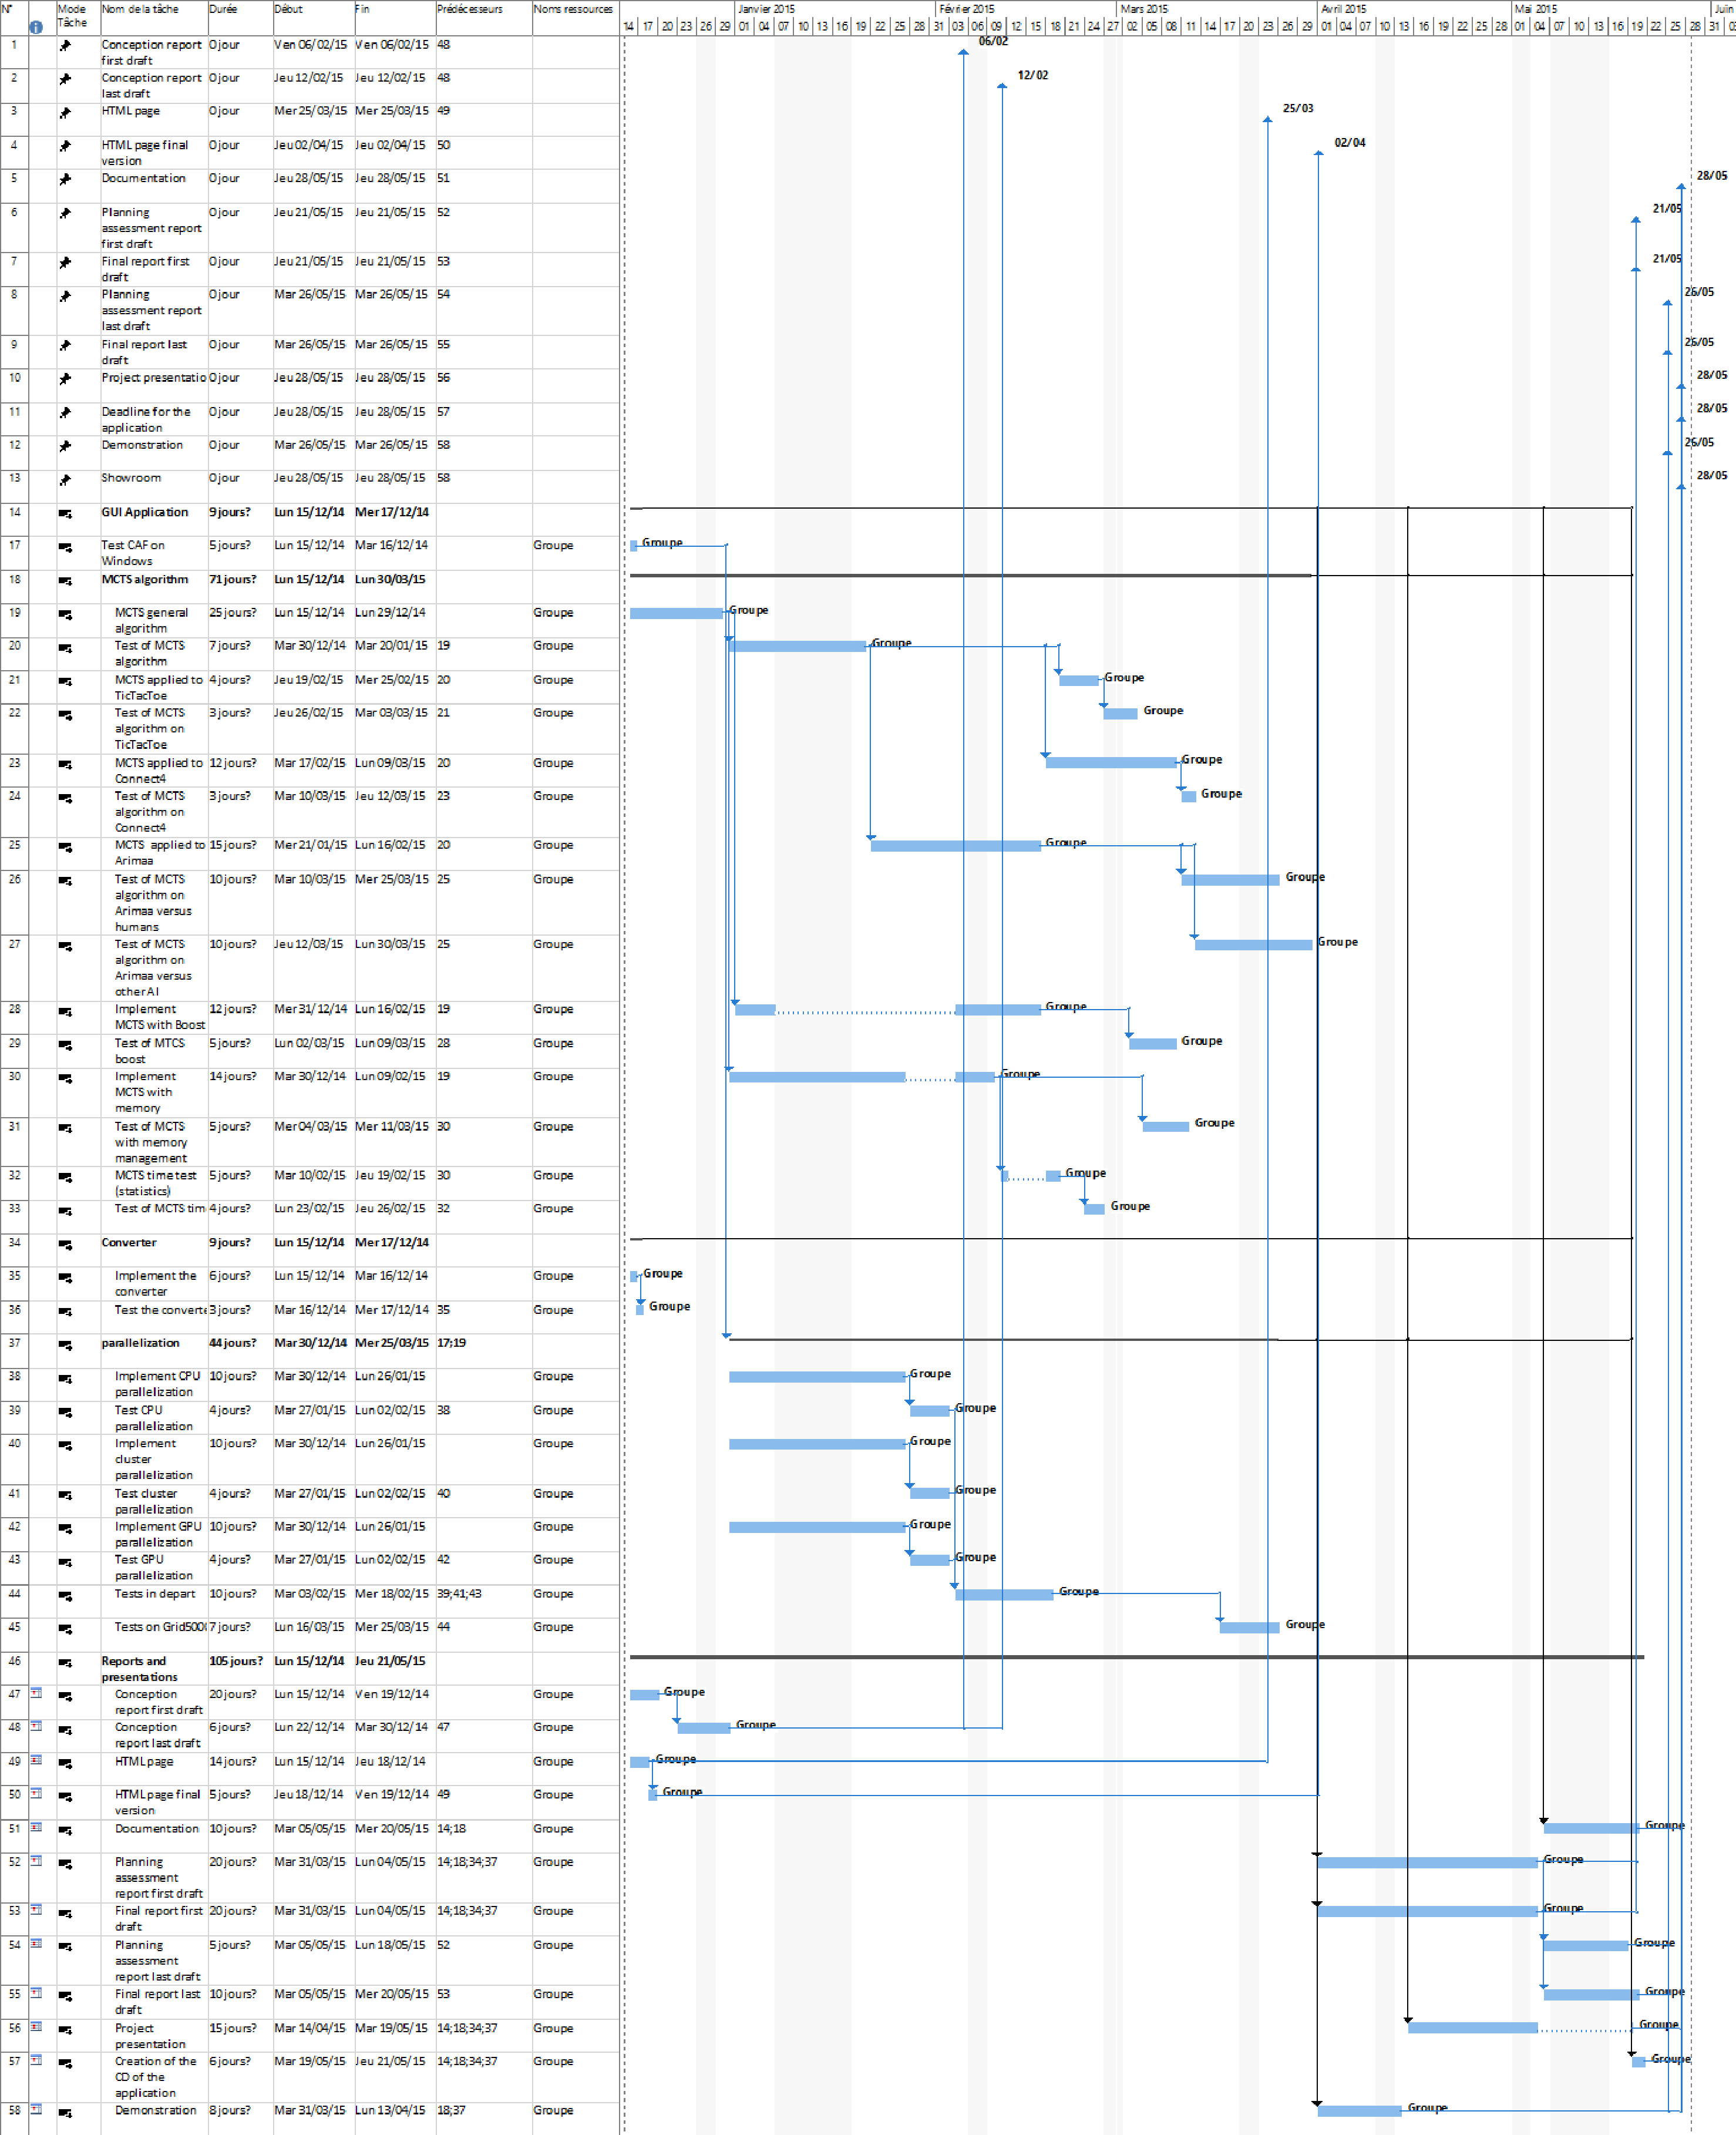
\includegraphics[angle = 90,scale = 0.60,viewport=0 0 1000 1625]{g.pdf}}
\caption[]{}
\end{center}
\end{figure}
\vspace*{\fill}

\begin{figure}[htb]
\ContinuedFloat
\begin{center}
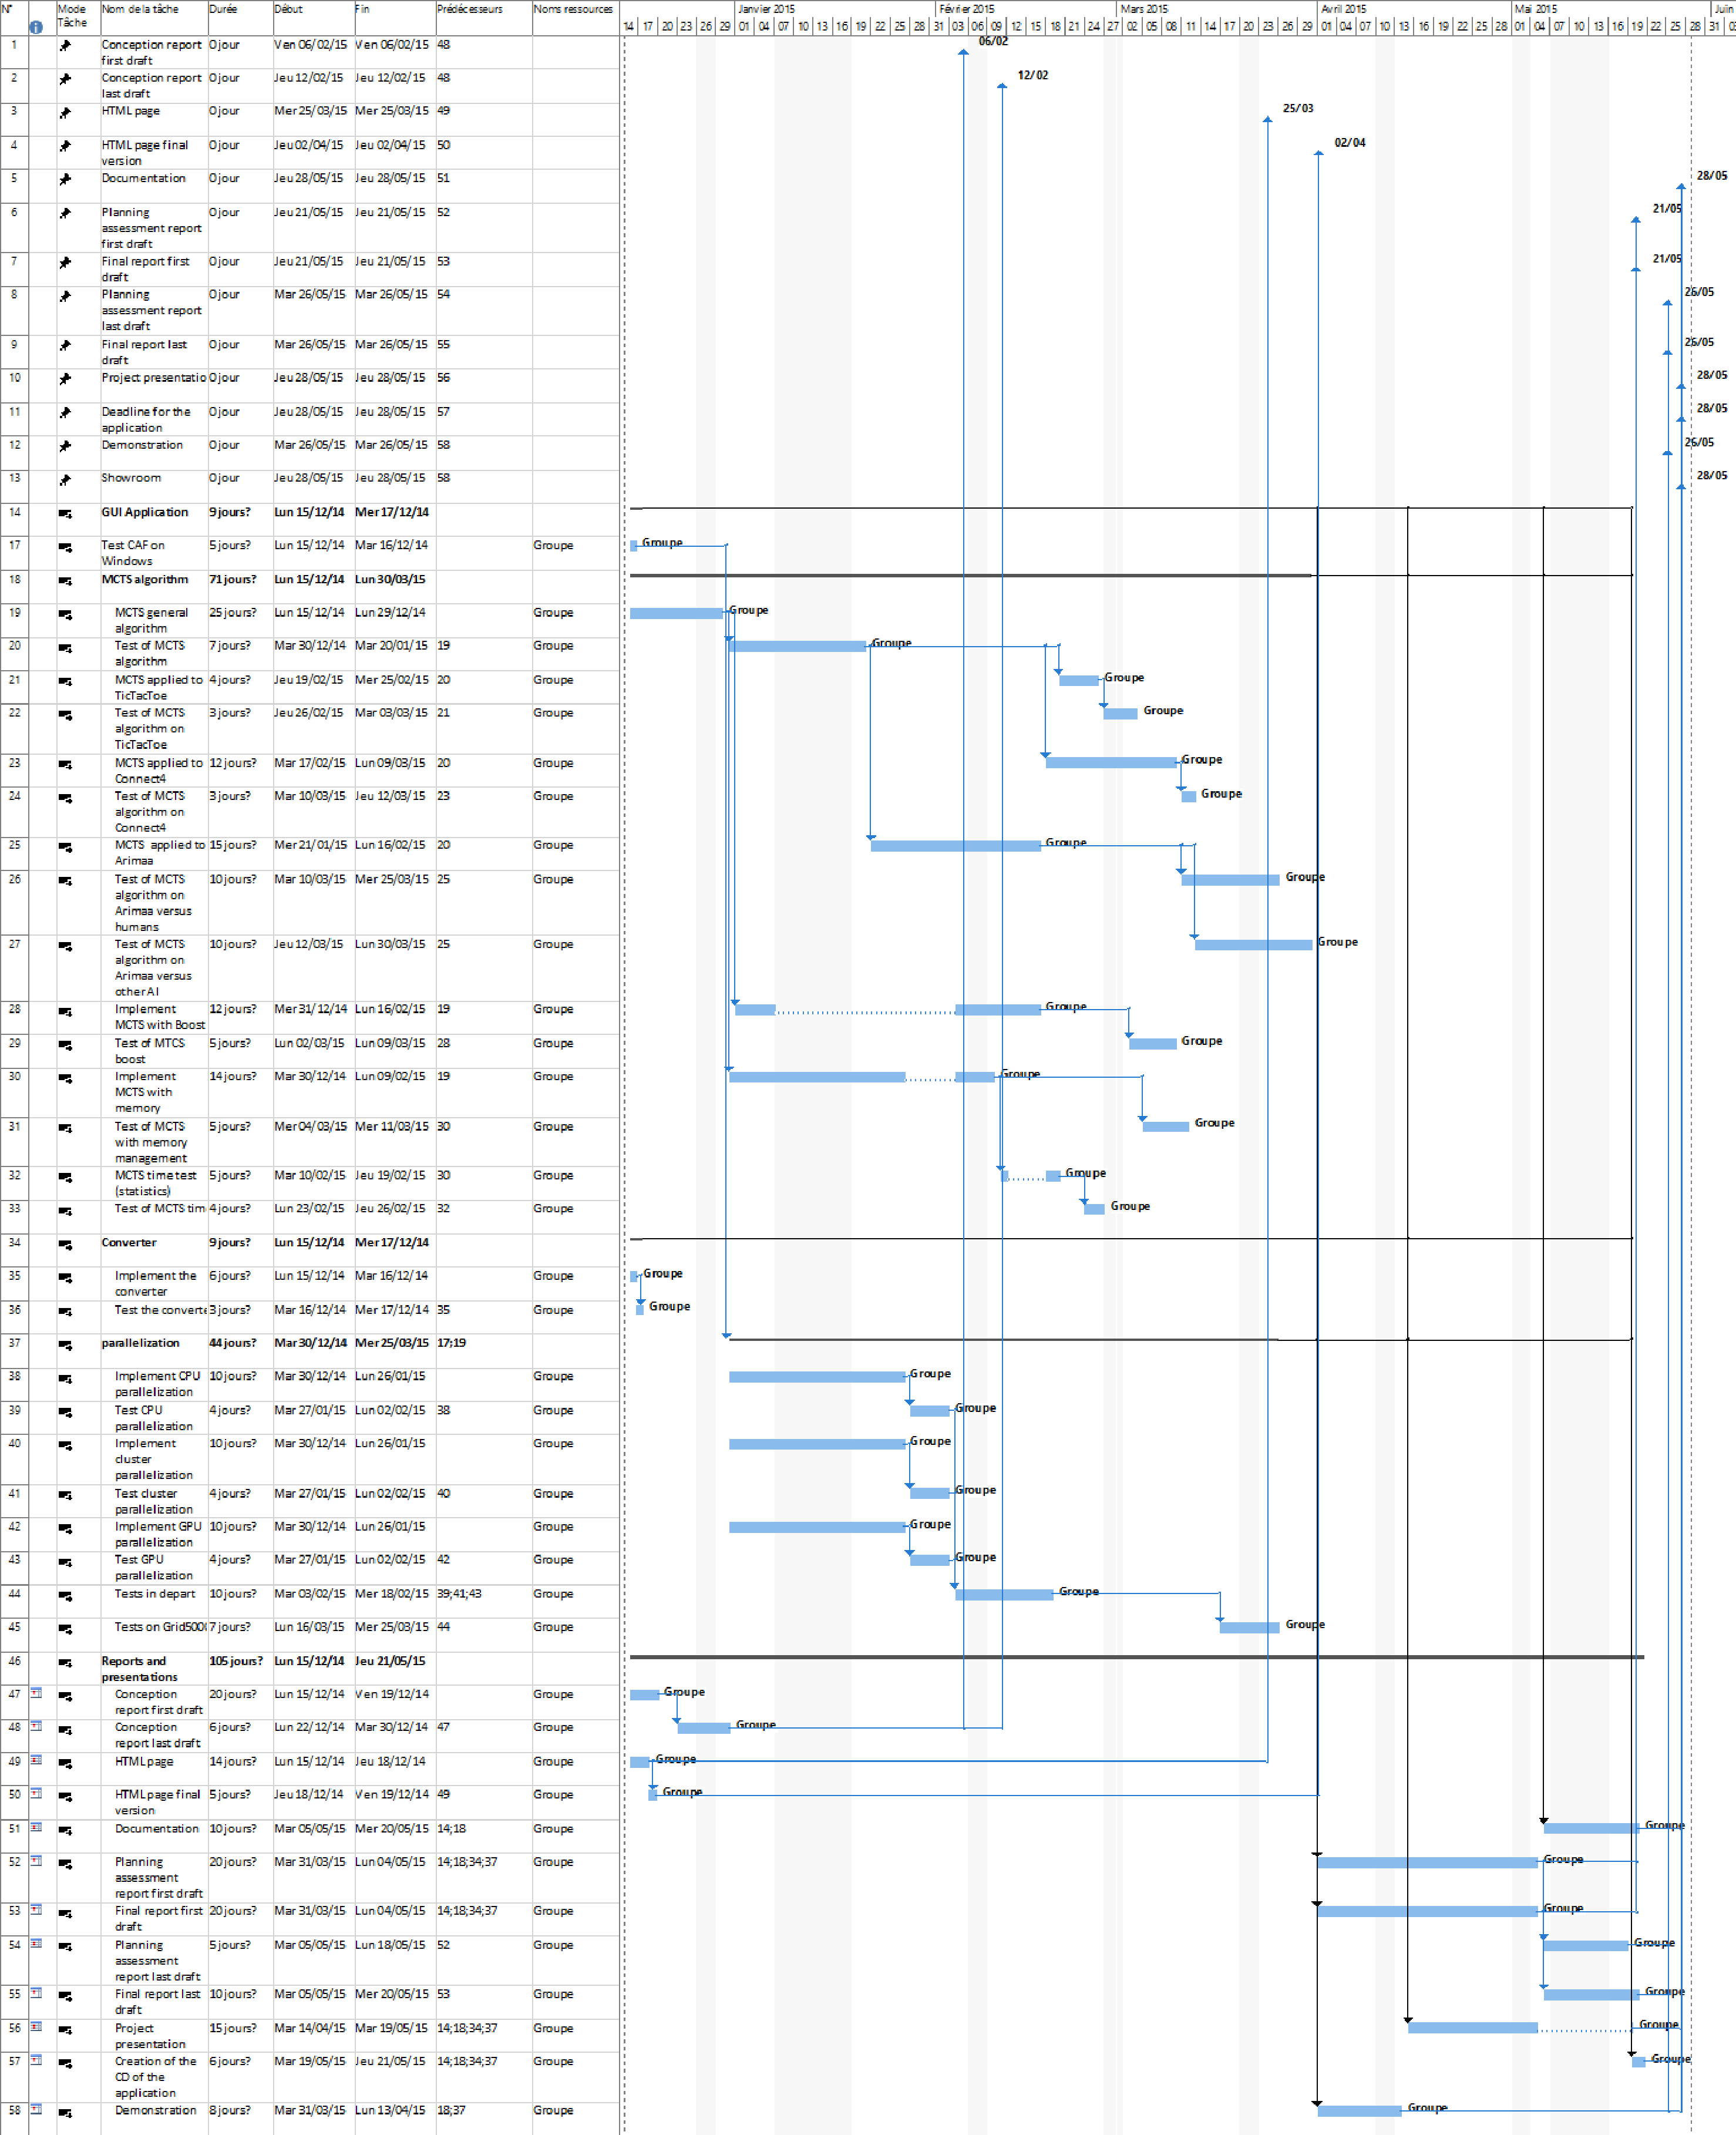
\includegraphics[totalheight=.5\textheight,
width=.7\textwidth,viewport=0 0 580 480]{g.pdf}
\end{center}
\caption[]{}
\end{figure}
\clearpage












\clearpage
sdhjfds

\end{document}
